\section{Teil}
beinhaltet folgende Foliensätze:

\begin{itemize}
    \item Teil 2: Systemanforderungen (Requirements Engineering)

\end{itemize}

% subsection
%-------------------------------------------------------------------------------------------
\subsection{Was versteht man unter einem Requirement?}

Ein \textbf{Requirement} definiert geforderte oder gewünschte Eigenschaften.

Betrifft \textbf{Funktionalität}, ein \textbf{Qualitätsmerkmal}, eine \textbf{Bedingung} oder \textbf{Fähigkeit}.

% subsection
%-------------------------------------------------------------------------------------------
\subsection{Was ist ein Stakeholder?}

Ist eine \textbf{Person} oder \textbf{Organisation}, welche Einfluss (direkt oder indirekt) auf die Anforderungen des Systems hat.

% subsection
%-------------------------------------------------------------------------------------------
\subsection{Wie kann man Requirements Engineering und Requirements Management unterscheiden?}

\textbf{Requirements Engineering}

\begin{itemize}
    \item Entwickeln der Anforderungsbasis.
    \item Analysieren, Ermitteln, Strukturieren, Spezifizieren von Anforderungen.
\end{itemize}

\textbf{Requirements Management}
\begin{itemize}
    \item Arbeiten mit Anforderungen.
    \item Dokumentieren, Ändern, Rückverfolgen, Versionieren von Anforderungen.
\end{itemize}

% subsection
%-------------------------------------------------------------------------------------------
\subsection{Wie werden Anforderungen angegeben?   ---nicht sicher---}

\textbf{Anforderung}
\begin{itemize}
    \item Geforderte Eigenschaft bezogen auf Produkt oder Entwicklung.
    \item Formal durch Merkmale und Ausprägungen ausdrücken.
    \item Repräsentiert ein Entwicklungsziel.
\end{itemize}

\textbf{Merkmal}
\begin{itemize}
    \item Beschreibt Bezugsobjekt der Anforderung (z.B. Namen).
\end{itemize}

\textbf{Ausprägung}
\begin{itemize}
    \item Bezeichnet den Sollwert für das Anforderungsmerkmal.
    \item Beinhaltet bei quantitativen Anforderungen einen Wertebereich und Einheit.
    \item Beinhaltet bei qualitativen Anforderungen einen verbalen Ausdruck.
\end{itemize}

\begin{figure}[H]
    \centering
    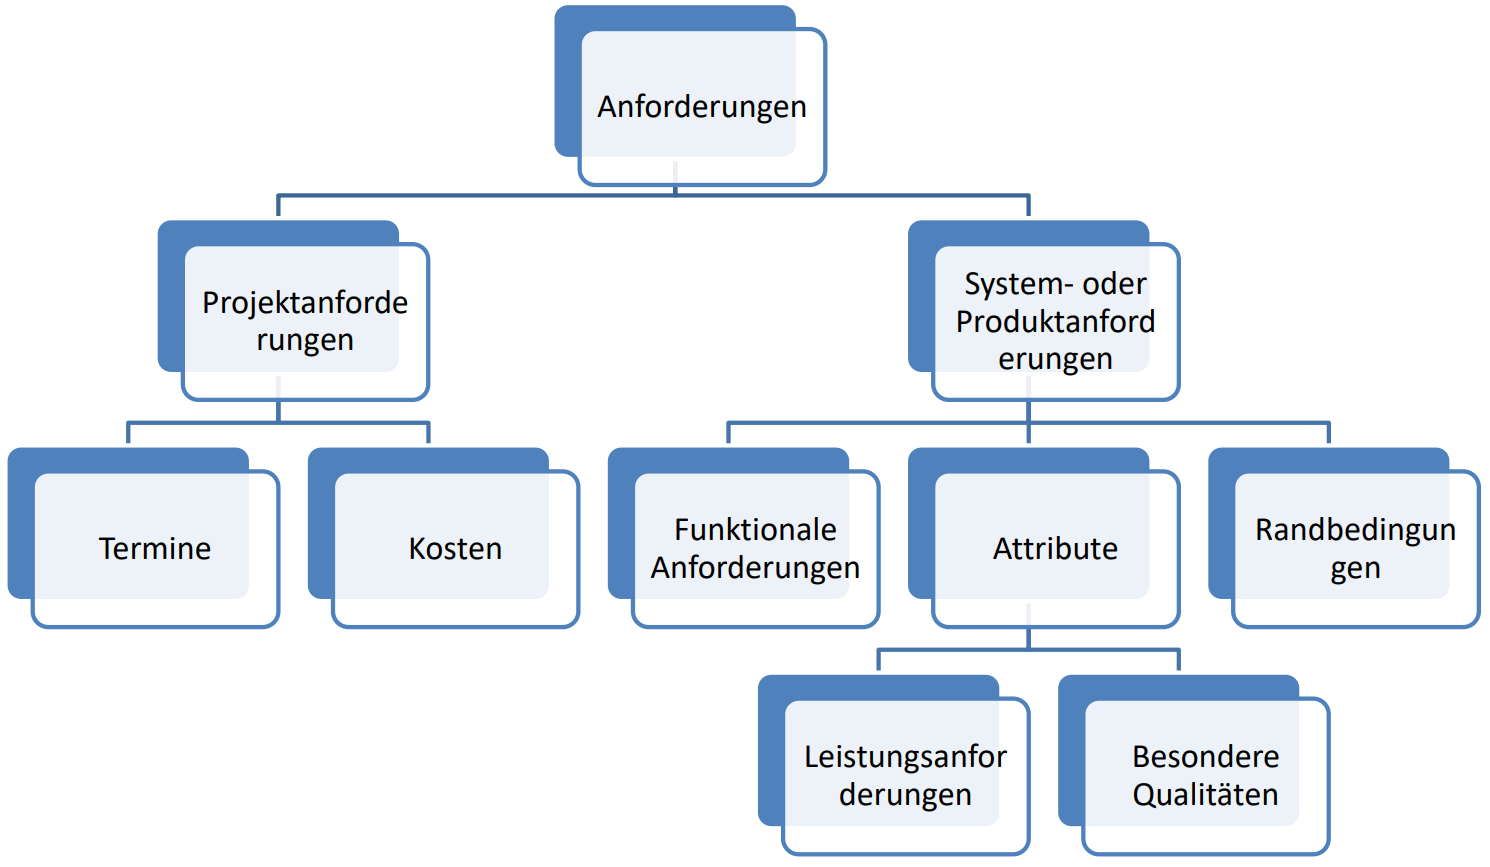
\includegraphics[width=0.7\linewidth]{Bilder/Teil2_KlassifikationAnforderungen.png}
    \caption{Klassifikation von Anforderungen}
\end{figure}

% subsection
%-------------------------------------------------------------------------------------------
\subsection{Nennen Sie Funktionale Anforderungen. (Zusatz!)}

Beschreiben funktionale Aspekte des Systems.

\begin{itemize}
    \item Fragestellung: \textbf{Was tut das System}
    \item Beschreibt Funktionen, Eingaben, Ausgaben (Daten, Fehlermeldungen, ...) des Systems.
    \item Beschreiben wichtige Systemzustände und das Verhalten des Systems.
    \item Bsp.: Der Alarm soll ausgelöst werden, sobald der Sensor das Zerbechen der Fensterscheibe detektiert.
\end{itemize}

% subsection
%-------------------------------------------------------------------------------------------
\subsection{Nennen Sie Nicht-Funktionale Anforderungen.}

\begin{itemize}
    \item \textbf{Technologische Anforderungen}
        \begin{itemize}
            \item schränken Lösungsraum des Systems ein.
            \item Definieren vorgegebene Lösungswege.
        \end{itemize}
    \item \textbf{Qualitätsanforderungen}
        \begin{itemize}
            \item Definieren die Qualität des Produktes.
        \end{itemize}
    \item \textbf{Anforderungen an Benutzeroberfläche}
        \begin{itemize}
            \item Anforderungen an die Bedienung des Produktes.
        \end{itemize}
    \item \textbf{Nebenprodukte}
        \begin{itemize}
            \item Notwendig für Funktion bzw. Verständnis des Produktes (z.B. Doku).
            \item Unterpunkt2
        \end{itemize}
    \item \textbf{Anforderungen an durchzuführende Tätigkeiten}
        \begin{itemize}
            \item Tätigkeiten, welche nach dem Entwicklungsprozess anfallen (z.B. Wartung)
        \end{itemize}
    \item \textbf{Rechtlich- Vertragliche Anforderungen}
        \begin{itemize}
            \item Anforderungen zwischen Vertragspartnern vor Entwicklungsbeginn.
        \end{itemize}
\end{itemize}


% subsection
%-------------------------------------------------------------------------------------------
\subsection{Was sind typischen Schritte im Requirements Engineering?}

\begin{itemize}
    \item Anforderungen \textbf{erheben} (z.B. Befragung von Stakeholdern)
    \item Anforderungen \textbf{dokumentieren} (z.B. Lastenheft)
    \item Anforderungen \textbf{verifizieren} (z.B. Hinblick auf Spezifikation)
    \item Anforderungen \textbf{validieren} (z.B. Hinblick auf Zweck oder Anforderungen)
    \item Anforderungen \textbf{verwalten} (z.B. Administrative Werkzeuge wie: Freigeben, Ändern, Rückverfolgen)
\end{itemize}

% subsection
%-------------------------------------------------------------------------------------------
\subsection{Nennen Sie Quellen für Anforderungen?}

\textbf{3 Teilbereiche zur Gewinnung von Anforderungen}
\begin{itemize}
    \item Identifizierung relevanter Anforderungsquellen
    \item Gewinnung von existierenden Anforderungen
    \item Entwicklung von innovativen Anforderungen
\end{itemize}

\textbf{Methoden}
\begin{itemize}
    \item Interviews
    \item Workshops
    \item Beobachtungen
    \item Schriftliche Befragung
    \item Perspektivenbasiertes Lesen
\end{itemize}

\begin{figure}[H]
    \centering
    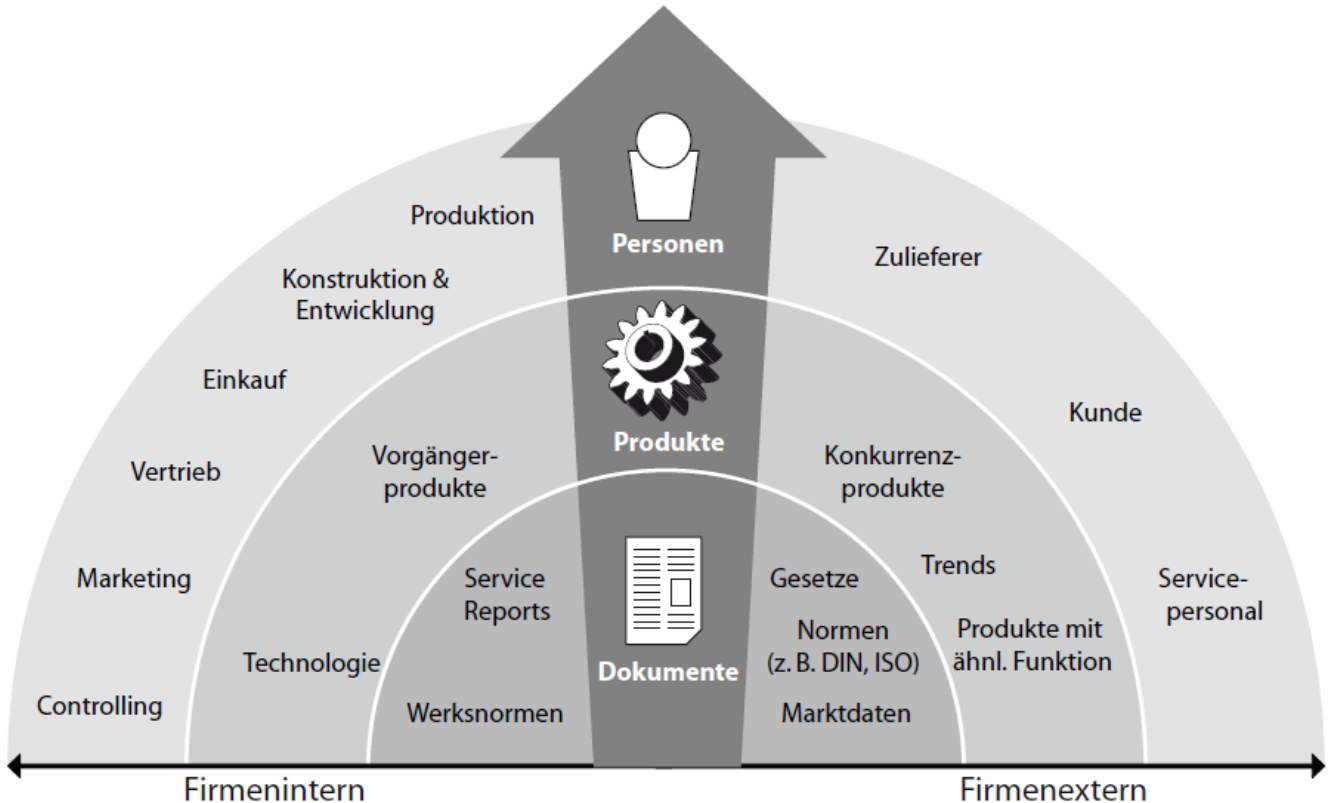
\includegraphics[width=0.7\linewidth]{Bilder/Teil2_QuellenAnforderungen.png}
    \caption{Klassifikation von Anforderungen}
\end{figure}

% subsection
%-------------------------------------------------------------------------------------------
\subsection{Was sind Qualitätskriterien für Anforderungen?}

\textbf{Smarte Anforderungen}
\begin{itemize}
    \item Spezifiziert
    \item Messbar
    \item Akzeptiert
    \item Realisierbar
    \item Terminiert
    \item Eindeutig
    \item Vollständig
    \item Bewertet
\end{itemize}

% subsection
%-------------------------------------------------------------------------------------------
\subsection{Was sind typische Bestandteile einer Anforderungsliste?}

\textbf{Inhalte der Anforderungsliste}
\begin{itemize}
    \item Forderungen
        \begin{itemize}
            \item Müssen erfüllt werden.
            \item Können auch als Mindset oder Maximalforderungen definiert.
        \end{itemize}
    \item Wünsche
        \begin{itemize}
            \item Sollen erfüllt werden.
            \item Aufgabenlösung auch ohne Erfüllung der Wünsche.
        \end{itemize}
    \item Quantitative Angaben
        \begin{itemize}
            \item Forderungen und Wünsche so weit wie möglich mit konkreten Werten angeben (Eindeutige Interpretation).
        \end{itemize}
    \item Qualitative Angaben
        \begin{itemize}
            \item Besondere Anforderungen oft ohne definierte Werte angegeben.
        \end{itemize}
    \item Administrative und ordnenden Angaben
        \begin{itemize}
            \item Benutzer
            \item Projektbezeichnung
            \item relevante Datum
            \item Ersteller
            \item Änderer
        \end{itemize}
\end{itemize}

% subsection
%-------------------------------------------------------------------------------------------
\subsection{Mit welcher Methode können Zielkonflikte erkannt werden und erklären Sie diese! }



\textbf{Methode : Korrelationsmatrix} \\

\textbf{Gründe für Korrelationsmatrix}
\begin{itemize}
    \item Bereinigung der Anforderungsliste um Inkonsistenzen und Redundanzen.
    \item Analyse von Wechselbeziehungen zwischen Anforderungen und Identifikation von Zielkonflikten.
    \item Priorisierung von Anforderungen.
\end{itemize}


\begin{itemize}
    \item Wechselbeziehung zwischen Anforderungen eintragen.
    \item Gewichtung zur Darstellung der Stärke der Abhängigkeit .
    \item Matrix oft symmetrisch.
\end{itemize}

\begin{figure}[H]
    \centering
    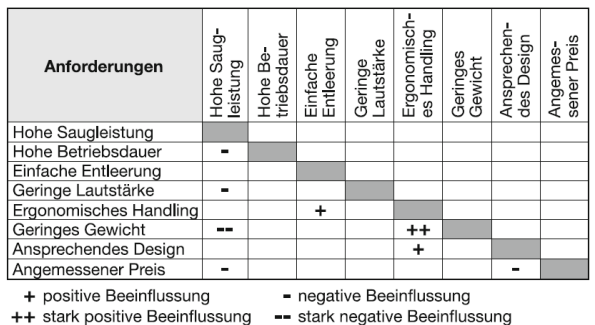
\includegraphics[width=0.7\linewidth]{Bilder/Teil2_Korrelationsmatrix_Beispiel.png}
    \caption{Beispiel Korrelationsmatrix}
\end{figure}